\section{Experiments}
\label{sec:experiments}

\subsection{Implementation Details}

% da3 setting
% Loss hyperparameters
% training settings (gpu, memory, batch size, lr)
We adopt DA3-GIANT \cite{lin2025da3} as our baseline. We follow DA3 to freeze the main encoder and the pre-trained depth/pose heads, optimizing only the Gaussian prediction head to maintain the powerful geometric priors of the foundation model. 
The Gaussian head predictions include 3D refinement for Gaussian means and other Gaussian attributes such as scales, rotations, and opacities. 
We train our model on $252 \times 252$ images for RealEstate10K (RE10K)~\cite{zhou2018stereo}, and $252 \times 448$ images for the DL3DV dataset~\cite{ling2024dl3dv}.
During each training iteration, we randomly sample 24 context views to construct the scene geometry and 8 spatially distinct target views for rendering supervision.
Training is conducted on 4 NVIDIA A100 40GB GPUs with a batch size of 1 per GPU, totaling $100,000$ iterations, while testing is performed on a single A100 40GB. Further details regarding our hyperparameters and model's weights update are provided in the \textit{Suppl}. 

% The loss weights are empirically determined as $\lambda_\text{geo}=0.1$ and $\lambda_\text{opa}=1.0$, while $\lambda_{s}$ is set to 0.1 for the LPIPS term.

% We employ the AdamW optimizer \cite{loshchilov2017adamw} with a learning rate of $2 \times 10^{-6}$ and a weight decay of $0.01$. 
% We use a OneCycleLR \cite{smith2019super} scheduler with a warm-up period of $2,000$ steps. 
% Training is conducted on 4 NVIDIA A100 GPUs with a batch size of 1 per GPU, totaling $100,000$ iterations. 
% In Rating-based Opacity Matching (ROM), we set the error decay rate $\gamma=5.0$ and the stability constant $\eta=10^{-7}$. 
% The loss weights are empirically determined as $\lambda_\text{geo}=0.1$ and $\lambda_\text{opa}=1.0$, while $\lambda_{s}$ is set to 0.1 for the LPIPS term. 

% In addition, we adopt the Exponential Moving Average (EMA) \cite{tarvainen2017ema} weights update strategy for stable training. Details of the weights update are in \textit{Suppl.}.


\subsection{Evaluation Protocol}
% We evaluate the NVS quality via Peak Signal-to-Noise Ratio (PSNR), Structural Similarity Index Measure (SSIM), and Learned Perceptual Image Patch Similarity (LPIPS)~\cite{zhang2018perceptual}. 
We evaluate the NVS quality via PSNR, SSIM, and LPIPS~\cite{zhang2018perceptual}. We adopt the evaluation protocol established by recent pose-free NVS literature~\cite{ye2024no, huang2025no, park2026ecosplat} on the RE10K dataset. This setting stratifies testing sequences based on the visual overlap ratios between the initial and terminal frames. We utilize sequences with overlap ratios of less than $10\%$. Furthermore, we evaluate the existing methods under wide-baseline conditions on the complex DL3DV dataset by constructing challenging context-target splits. Specifically, we constrain the frame intervals between the starts and ends of the testing sequences to 90, 150, and 150 frames for the 12-, 24-, and 36-view settings, respectively. Target views are uniformly sampled across these sequences, while context views are randomly drawn from the mutually exclusive remaining frames. To analyze models' robustness, we perform the cross-dataset generalization evaluation on the ACID dataset \cite{infinite_nature_2020} as in \cite{chen2024mvsplat, huang2025no}, by utilizing the testing splits from \cite{park2026ecosplat}. Similar to prior pose-free approaches \cite{fu2024colmap, huang2025no, ye2024no,ye2026yonosplat}, we adopt the test-time pose optimization for ground truth alignment for all pose-free NVS baselines.


\subsection{NVS Performance Evaluation}

\begin{table*}[t]
\begin{center}
    \scriptsize
    \caption{Quantitative comparison of NVS performance on the RE10K dataset~\cite{zhou2018stereo} under various input-view settings. \best{Bold} indicates the best performance. OOM indicates out-of-memory inference error.}
    \vspace{-3mm}
    \resizebox{\linewidth}{!}{ 
        \setlength{\tabcolsep}{3pt}
\renewcommand{\arraystretch}{1.2}

\centering
\scriptsize
\begin{tabular}{ll | ccc | ccc | ccc}
\toprule
\multicolumn{2}{c|}{\multirow{2}{*}{Methods}} & \multicolumn{3}{c|}{12 Views} & \multicolumn{3}{c|}{24 Views} & \multicolumn{3}{c}{36 Views} \\
\cmidrule(lr){3-5} \cmidrule(lr){6-8} \cmidrule(lr){9-11}
& & PSNR$\uparrow$ & SSIM$\uparrow$ & LPIPS$\downarrow$ & PSNR$\uparrow$ & SSIM$\uparrow$ & LPIPS$\downarrow$ & PSNR$\uparrow$ & SSIM$\uparrow$ & LPIPS$\downarrow$ \\
\midrule
\multirow{3}{*}{\shortstack{w/ \\ Pose}} 
& MonoSplat~\cite{liu2025monosplat} (CVPR25) & 18.16 & 0.663 & 0.336 & 16.66 &	0.593 & 0.391 & 15.79 & 0.551 & 0.424 \\ 
& MVSplat~\cite{chen2024mvsplat} (ECCV24) & 17.98 & 	0.638 & 0.357 & 17.27 & 0.609 & 0.379  & OOM & OOM	& OOM \\
& DepthSplat~\cite{xu2025depthsplat} (CVPR25) & \second{22.56} & \second{0.793} & \second{0.200}  & 21.00 & \second{0.734} & 0.248  & 19.60 & 0.676 & 0.296 \\
% & Zpressor~\cite{wang2025zpressor} & 23.15 & 	0.817 & 0.188 & 23.53 & 0.812 & 	0.181 & 23.41 & 0.809 & 0.185 \\
\midrule
\multirow{7}{*}{\shortstack{Pose- \\ free}} 
& NoPoSplat~\cite{ye2024no} (ICLR25) & 17.15 & 0.571 & 0.437 &  17.10 & 	0.570 & 0.443  & 17.09 & 0.570 & 0.446 \\
& AnySplat~\cite{jiang2025anysplat} (SIGGRAPHAsia25) & 18.69 & 0.591 & 0.273 & 19.15 & 0.610 & 0.257 & 19.31 & 0.615 & 0.251 \\
& WorldMirror~\cite{liu2025worldmirror} (arXiv25) & 21.23	 & 0.707 & 0.267 & 21.08 & 0.701 & 0.274 & 20.98 & \second{0.699} & 0.275 \\
& SPFSplat~\cite{huang2025no} (ICCV25) & 21.57 & 0.701 & 0.254 & 21.32 & 0.694 & 0.266 & 21.17 & 0.689 & 0.273 \\
& YoNoSplat~\cite{ye2026yonosplat} (ICLR26) & 21.62 & 0.679 & 0.229 & \second{21.63} & 0.679 & \second{0.227} & \second{21.60} & 0.681 & \second{0.226} \\
& DA3~\cite{lin2025da3} (ICLR26) & 20.78 & 0.715 & 0.250 & 21.06 & 0.710 & 0.254 & 21.11 & 0.684 & 0.274 \\
& \textbf{AirSplat(Ours)} & \best{23.08} & \best{0.799} & \best{0.190} & \best{23.77} & \best{0.814} & \best{0.178} & \best{23.94} & \best{0.815} & \best{0.179} \\
\bottomrule
\end{tabular}
    }
\label{table:main_re10k}
\end{center}
\end{table*}

\begin{figure*}[t]
    \centering
    \includegraphics[width=\linewidth]{figures/qualitative_re10k_main.pdf}
    \vspace{-5mm}
    \caption{Qualitative comparison of NVS performance on RE10K dataset \cite{zhou2018stereo}.}
    \vspace{-3mm}
    \label{fig:qualitative_re10k_main}
\end{figure*}

\noindent \textbf{Comparison on RE10K.}
We evaluate our model on the RE10K dataset to verify its scalability and robustness in large-scale indoor and outdoor environments. 
As shown in Table~\ref{table:main_re10k}, our proposed AirSplat achieves SOTA performance among pose-free methods, demonstrating superior NVS quality.
Most notably, our method not only outperforms existing pose-free benchmarks such as YoNoSplat \cite{ye2026yonosplat} and WorldMirror \cite{liu2025worldmirror} by significant margins, but also remarkably exceeds the performance of several pose-required methods \cite{liu2025monosplat, xu2025depthsplat}. 
These results indicate that our approach effectively compensates for the absence of ground-truth camera poses by leveraging powerful geometric reasoning based on our SCPA and ROM, ultimately leading to more accurate and sharper novel view renderings compared to prior pipelines.
In Fig.~\ref{fig:qualitative_re10k_main}, our proposed AirSplat successfully preserves challenging high-frequency details, such as thin structures, while aggressively suppressing the floater artifacts and blurry regions that frequently degrade the outputs of prior methods.

\begin{table*}[t]
\begin{center}
    \scriptsize
    \caption{Quantitative comparison of NVS performance on the DL3DV dataset~\cite{ling2024dl3dv} under various input-view settings.}
    \vspace{-3mm}
    \resizebox{\linewidth}{!}{ 
        \setlength{\tabcolsep}{3pt}
\renewcommand{\arraystretch}{1.2}

\begin{tabular}{ll | ccc | ccc | ccc}
\toprule
\multicolumn{2}{c|}{\multirow{2}{*}{Methods}} & \multicolumn{3}{c|}{12 Views} & \multicolumn{3}{c|}{24 Views} & \multicolumn{3}{c}{36 Views} \\
\cmidrule(lr){3-5} \cmidrule(lr){6-8} \cmidrule(lr){9-11}
& & PSNR$\uparrow$ & SSIM$\uparrow$ & LPIPS$\downarrow$ & PSNR$\uparrow$ & SSIM$\uparrow$ & LPIPS$\downarrow$ & PSNR$\uparrow$ & SSIM$\uparrow$ & LPIPS$\downarrow$ \\
\midrule
\multirow{2}{*}{\shortstack{w/ \\ Pose}} 
& MVSplat~\cite{chen2024mvsplat} (ECCV24) & 21.55 & \second{0.729} & 0.239 & OOM & OOM & OOM & OOM & OOM & OOM \\
& DepthSplat~\cite{xu2025depthsplat} (CVPR25) & \second{22.14} & 0.725 & \second{0.221} & \second{19.87} & \second{0.695} & \second{0.274} & 18.69 & 0.643 & 0.330 \\
% & Zpressor~\cite{wang2025zpressor} & 20.82 & 0.691 & 0.233 & 19.67 & 0.656 & 0.280 & 19.73 & 0.658 & 0.279 \\ 
\midrule
\multirow{6}{*}{\shortstack{Pose- \\ free}} 
& NoPoSplat~\cite{ye2024no} (ICLR25)& 16.13 & 0.447 & 0.497 & 14.73 & 0.392 & 0.603 & 13.82 & 0.365 & 0.640 \\
& AnySplat~\cite{jiang2025anysplat} (SIGGRAPHAsia25) & 18.72 & 0.551 & 0.310 & 18.40 & 0.533 & 0.333 & 18.36 & 0.529 & 0.337 \\
& WorldMirror~\cite{liu2025worldmirror} (arXiv25) & 20.44	& 0.625	& 0.278 & 19.78 & 0.594 & 0.312 & \second{19.67} & \second{0.589} & \second{0.316} \\
& YoNoSplat~\cite{ye2026yonosplat} (ICLR26) & 17.73 & 0.481 & 0.430 & 16.77 & 0.451 & 0.490 & 16.56 & 0.446 & 0.502 \\
& DA3~\cite{lin2025da3} (ICLR26) & 20.74 & 0.691 & 0.242 & 20.51 & 0.644 & 0.274 & 20.38 & 0.642 & 0.285 \\
& \textbf{AirSplat(Ours)} & \best{22.50} & \best{0.747} & \best{0.207} & \best{22.22} & \best{0.735} & \best{0.217} & \best{22.07} & \best{0.730} & \best{0.225} \\
\bottomrule
\end{tabular}
    }
\label{table:main_dl3dv}
\end{center}
\end{table*}

\begin{figure*}[t]
    \centering
    \includegraphics[width=\linewidth]{figures/qualitative_dl3dv_main.pdf}
    \vspace{-5mm}
    \caption{Qualitative comparison of NVS performance on DL3DV dataset \cite{ling2024dl3dv}.}
    \vspace{-3mm}
    \label{fig:qualitative_dl3dv_main}
\end{figure*}

\noindent \textbf{Comparison on DL3DV.}
Table \ref{table:main_dl3dv} reports the quantitative NVS performance on the DL3DV dataset compared to recent SOTA methods \cite{chen2024mvsplat, xu2025depthsplat, ye2024no, jiang2025anysplat, liu2025worldmirror, ye2026yonosplat}. 
Our AirSplat consistently achieves superior performance across all evaluation settings (12, 24, 36 views) in PSNR, SSIM, and LPIPS metrics.
Notably, in the 12-view setting, despite being a pose-free approach, our method surpasses the established SOTA pose-required method, DepthSplat \cite{xu2025depthsplat}. 
Moreover, AirSplat outperforms the baseline DA3 by a \textit{significant} margin of {+1.76 dB} in PSNR and reduces LPIPS by 14.4\%. 
While base 3D-VS-VFMs (e.g., WorldMirror~\cite{liu2025worldmirror}, DA3~\cite{lin2025da3}) are robust with increased input views, applying our proposed training strategy significantly amplifies DA3's rendering quality, yielding substantial margins in all metrics. 
% These results highlight our approach's effectiveness in achieving high-fidelity NVS without relying on ground-truth camera poses.
Furthermore, as shown in Fig.~\ref{fig:qualitative_dl3dv_main}, our AirSplat synthesizes clean, floater-free novel views across varying input densities.
Specifically, in the third row, while other methods fail to capture thin structures, our AirSplat accurately reconstructs the sharp geometry of the pole, further validating the robust multi-view consistency and structural integrity enforced by our pipeline.

\begin{table*}[t]
\begin{center}
    \scriptsize
    \caption{Cross-dataset generalization performance under various input-view settings. We evaluate the zero-shot performance on the ACID dataset~\cite{infinite_nature_2020}.}
    \vspace{-3mm}
    \resizebox{\linewidth}{!}{ 
        \setlength{\tabcolsep}{3pt}
\renewcommand{\arraystretch}{1.2}

\centering
\scriptsize
\begin{tabular}{ll | ccc | ccc | ccc}
\toprule
\multicolumn{2}{c|}{\multirow{2}{*}{Methods}} & \multicolumn{3}{c|}{16 Views} & \multicolumn{3}{c|}{20 Views} & \multicolumn{3}{c}{24 Views} \\
\cmidrule(lr){3-5} \cmidrule(lr){6-8} \cmidrule(lr){9-11}
& & PSNR$\uparrow$ & SSIM$\uparrow$ & LPIPS$\downarrow$ & PSNR$\uparrow$ & SSIM$\uparrow$ & LPIPS$\downarrow$ & PSNR$\uparrow$ & SSIM$\uparrow$ & LPIPS$\downarrow$ \\
\midrule
\multirow{3}{*}{\shortstack{w/ \\ Pose}} 
& MonoSplat~\cite{liu2025monosplat} (CVPR25) & 17.81 & 0.642 & 0.345 & 17.48 & 0.625 & 0.361 & 17.23 & 0.611 & 0.372 \\ 
& MVSplat~\cite{chen2024mvsplat} (ECCV24) & 18.19 & 	0.502 & 0.376 & 18.12 & 0.500 &	0.379 & 18.09 & 0.500 & 0.379 \\
& DepthSplat~\cite{xu2025depthsplat} (CVPR25) & 20.41 & 0.713 & 0.268  & 19.92 & 0.694 & 0.286 & 19.78 & 0.688	 & 0.289 \\
% & Zpressor~\cite{wang2025zpressor} & 23.15 & 	0.817 & 0.188 & 23.53 & 0.812 & 	0.181 & 23.41 & 0.809 & 0.185 \\
\midrule
\multirow{7}{*}{\shortstack{Pose- \\ free}} 
& NoPoSplat~\cite{ye2024no} (ICLR25) & 22.30	 & 0.668 & 0.286 &  22.24 & 0.666 & 0.288 & 22.25 & 0.666 & 0.288  \\
& AnySplat~\cite{jiang2025anysplat} (SIGGRAPHAsia25) & 21.89 & 0.615	& 0.275 & 22.05 & 0.622 & 0.256 & 21.96	 & 0.619 & 	0.258 \\
& WorldMirror~\cite{liu2025worldmirror} (arXiv25) & 22.15 & 0.646 & 0.275 & 22.20	& 0.650 & 0.275 & 22.34	 & 0.658 & 0.273 \\
& SPFSplat~\cite{huang2025no} (ICCV25) & \second{24.58} & \second{0.725} & \second{0.218} & \second{24.49} & \second{0.722} & \second{0.221} & \second{24.40} & \second{0.720 }& 	\second{0.222} \\
& YoNoSplat~\cite{ye2026yonosplat} (ICLR26) & 22.49 & 0.641 & 0.270 & 22.48 & 0.641 & 0.271 & 22.47 & 0.642 & 0.272 \\
& DA3~\cite{lin2025da3} (ICLR26) & 22.13 & 0.687 & 0.272 & 23.21 & 0.690 & 0.262 & 23.31 & 0.694 & 0.262 \\
& \textbf{AirSplat(Ours)} & \best{25.96} & \best{0.796} & \best{0.188} & \best{26.21} & \best{0.803} & \best{0.178} & \best{26.42} & \best{0.813} & \best{0.176} \\
\bottomrule
\end{tabular}



    }
\label{table:main_acid}
\end{center}
\end{table*}

\noindent \textbf{Cross Dataset Generalization.}
Following \cite{huang2025no, park2026ecosplat}, we conduct a cross-dataset evaluation at a resolution of $252\times252$ on the ACID dataset. 
All models were evaluated using 16, 20, and 24 input views without further fine-tuning. 
As shown in Table~\ref{table:main_acid}, our method achieves the highest performance across all metrics, significantly outperforming both pose-free and pose-required baselines.
Notably, in this zero-shot setting, our model maintains a substantial lead over other pose-free NVS methods such as SPFSplat \cite{huang2025no}, YoNoSplat \cite{ye2026yonosplat}, and 3D-VS-VFMs~\cite{liu2025worldmirror, lin2025da3}.
This superior performance in unseen environments demonstrates that our AirSplat does not merely overfit to the training distribution but instead learns highly generalizable geometric representations and robust view-consistency, effectively bridging the gap between pose-free and pose-dependent NVS.

% \begin{table*}[t]
% \begin{center}
%     \scriptsize
%     \caption{Ablation study on our SCPA and ROM. NVS performance comparison on the RE10K dataset~\cite{zhou2018stereo} under 12 input views.}
%     \setlength{\tabcolsep}{6pt}
\renewcommand{\arraystretch}{1.2}

\begin{tabular}{l | cccc}
\toprule
Methods & PSNR$\uparrow$ & SSIM$\uparrow$ & LPIPS$\downarrow$ \\
\midrule
Baseline (DA3 \cite{lin2025da3})  & 20.78 & 0.715 & 0.250 \\
Baseline + Context-only Training & 21.27 & 0.745 & 0.253 \\
Baseline + Context-Target Training & 21.63 & 0.761 & 0.241 \\
Baseline + Context-Target w/ SPCA Training & 22.60 & 0.776 & 0.215 \\
Baseline + ROM & 22.41 & 0.769 & 0.211\\
\textbf{Ours (Full)} & \textbf{23.08} & \textbf{0.799}	& \textbf{0.190} \\
\bottomrule
\end{tabular}

% \label{table:abl_main}
% \end{center}
% \end{table*}

\begin{figure}[t]
    \centering
    % ---------------------------------------------------
    % LEFT SIDE: The Figure
    % ---------------------------------------------------
    \begin{minipage}{0.43\textwidth}
        \centering
        % Replace with your actual image
        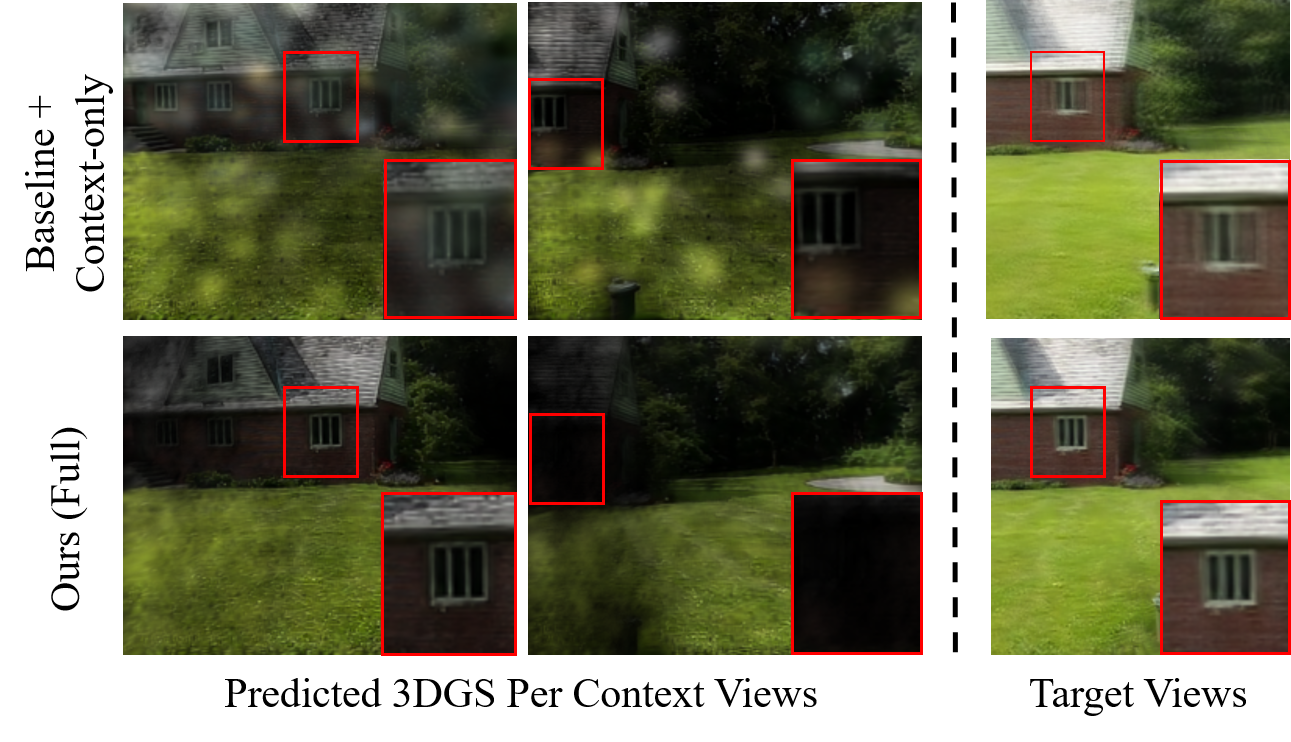
\includegraphics[width=\linewidth]{figures/rom_ablation.png} 
        \vspace{-5mm}
        \caption{Visualization of the `floaters' compression in the predicted 3DGS per context  views.}
        \vspace{-3mm}
        \label{fig:rom_ablation}
    \end{minipage}\hfill % \hfill pushes them apart to the edges
    % ---------------------------------------------------
    % RIGHT SIDE: The Table
    % ---------------------------------------------------
    \begin{minipage}{0.54\textwidth}
        \centering
        % This critical trick tells LaTeX to treat the following caption as a Table caption, 
        % even though we are inside a figure environment.
        \makeatletter\def\@captype{table}\makeatother
        
        \caption{Ablation study on our SCPA and ROM. NVS performance comparison on the RE10K dataset under 12 input views.}
        \label{table:abl_main}
        
        % We use resizebox to ensure the table never bleeds out of its half-page minipage
        \resizebox{\linewidth}{!}{
            \setlength{\tabcolsep}{6pt}
\renewcommand{\arraystretch}{1.2}

\begin{tabular}{l | cccc}
\toprule
Methods & PSNR$\uparrow$ & SSIM$\uparrow$ & LPIPS$\downarrow$ \\
\midrule
Baseline (DA3 \cite{lin2025da3})  & 20.78 & 0.715 & 0.250 \\
Baseline + Context-only Training & 21.27 & 0.745 & 0.253 \\
Baseline + Context-Target Training & 21.63 & 0.761 & 0.241 \\
Baseline + Context-Target w/ SPCA Training & 22.60 & 0.776 & 0.215 \\
Baseline + ROM & 22.41 & 0.769 & 0.211\\
\textbf{Ours (Full)} & \textbf{23.08} & \textbf{0.799}	& \textbf{0.190} \\
\bottomrule
\end{tabular}

        }
        \vspace{-3mm}
    \end{minipage}
\end{figure}

\subsection{Ablation Study}

In Table~\ref{table:abl_main}, we conduct an ablation study to evaluate the individual contributions of our proposed components: Self-Consistent Pose Alignment (SCPA) and Rating-based Opacity Matching (ROM) on the RE10K dataset \cite{zhou2018stereo}.

\noindent \textbf{Effectiveness of SCPA.}
The baseline model, DA3~\cite{lin2025da3}, shows limited performance (PSNR: 20.78, SSIM: 0.715), which underperforms the pose-free NVS methods \cite{liu2025worldmirror, ye2024no, ye2026yonosplat}. 
As discussed in Sec.~\ref{sec:scpa}, implementing a context-only training strategy yields only a marginal improvement over the baseline (reaching 21.27 dB PSNR), inherently limited by the absence of novel target views supervision. While adopting a naive context-target sampling strategy elevates this performance to 21.63 dB, the model remains fundamentally bottlenecked by the pose-geometry discrepancy. This uncorrected spatial misalignment ultimately results in structurally degraded 3D Gaussian primitives and blurry target renderings. Integrating our SCPA results in a significant performance leap, reaching 22.60 dB (+$0.97$ dB over context-target). 
The reduction in LPIPS from 0.250 (Baseline) to 0.215 indicates that SCPA effectively restores high-frequency details by ensuring a geometrically consistent rendering path during training.

\noindent \textbf{Effectiveness of ROM.}
The integration of Rating-based Opacity Matching (ROM) independently improves the baseline to 22.41 dB PSNR. This validates the necessity of local structural consensus for high-fidelity synthesis. As illustrated in Fig.~\ref{fig:main_architecture}, ROM acts as a "geometric filter" by matching the student's predicted opacity $\alpha$ with the teacher's geometric rating $\tilde{y}$. The improvement in perceptual metrics confirms that ROM effectively prunes floaters via opacity compression. 
By explicitly penalizing spatial inconsistencies, ROM ensures that only geometrically valid structures contribute to the final rendering.
As shown in Fig.~\ref{fig:rom_ablation}, AirSplat learns from ROM to suppress inconsistent geometry of complex regions (e.g., the window structures highlighted in red boxes).
The `Baseline + Context-only' variant produces noisy `floaters' at each context view's 3DGS estimation, resulting in severe blurring artifacts.
On the other hand, our full model assigns near-zero opacity for these inconsistent primitives, resulting in sharp and high-quality reconstructions for target views. 
% $\alpha=0$

\noindent \textbf{Full Model.}
Our full model, AirSplat, which combines both SCPA and ROM, achieves the best performance across all metrics, yielding a 25\% improvement in perceptual scores compared to naive fine-tuning. The synergy between global pose alignment and local structural refinement allows our framework to synthesize sharp, consistent novel views from uncalibrated context images. These results validate our core hypothesis that decoupling the pose errors from geometry optimization, complemented by teacher-driven consistency feedback, is essential for robust feed-forward NVS.